\chapter{Results}
This chapter aims to explore the operational boundaries of the chemical components in a Petri dish environment, focusing on the size limitations of the coincidence detector and the light sensitivity of a chemical diode.

The main objectives of the experiments are to find out the bounds and limitations of different chemical components in order to determine the feasibility of using them in a real-world environment.

\section{Size Limitations of the Coincidence Detector}
The goal here is to find a way to measure the size of the coincidence detector in real life, for which there is currently no data. The size of the coincidence detector is crucial for the design of the Petri dish, as it determines the minimum size of the Petri dish required to accommodate the detector. 

Creating the coincidence detector is covered in Appendix \ref{chap:creating-detector}, the final component is illustrated in Figure \ref{fig:and-gate}.


\begin{figure}
    \centering
    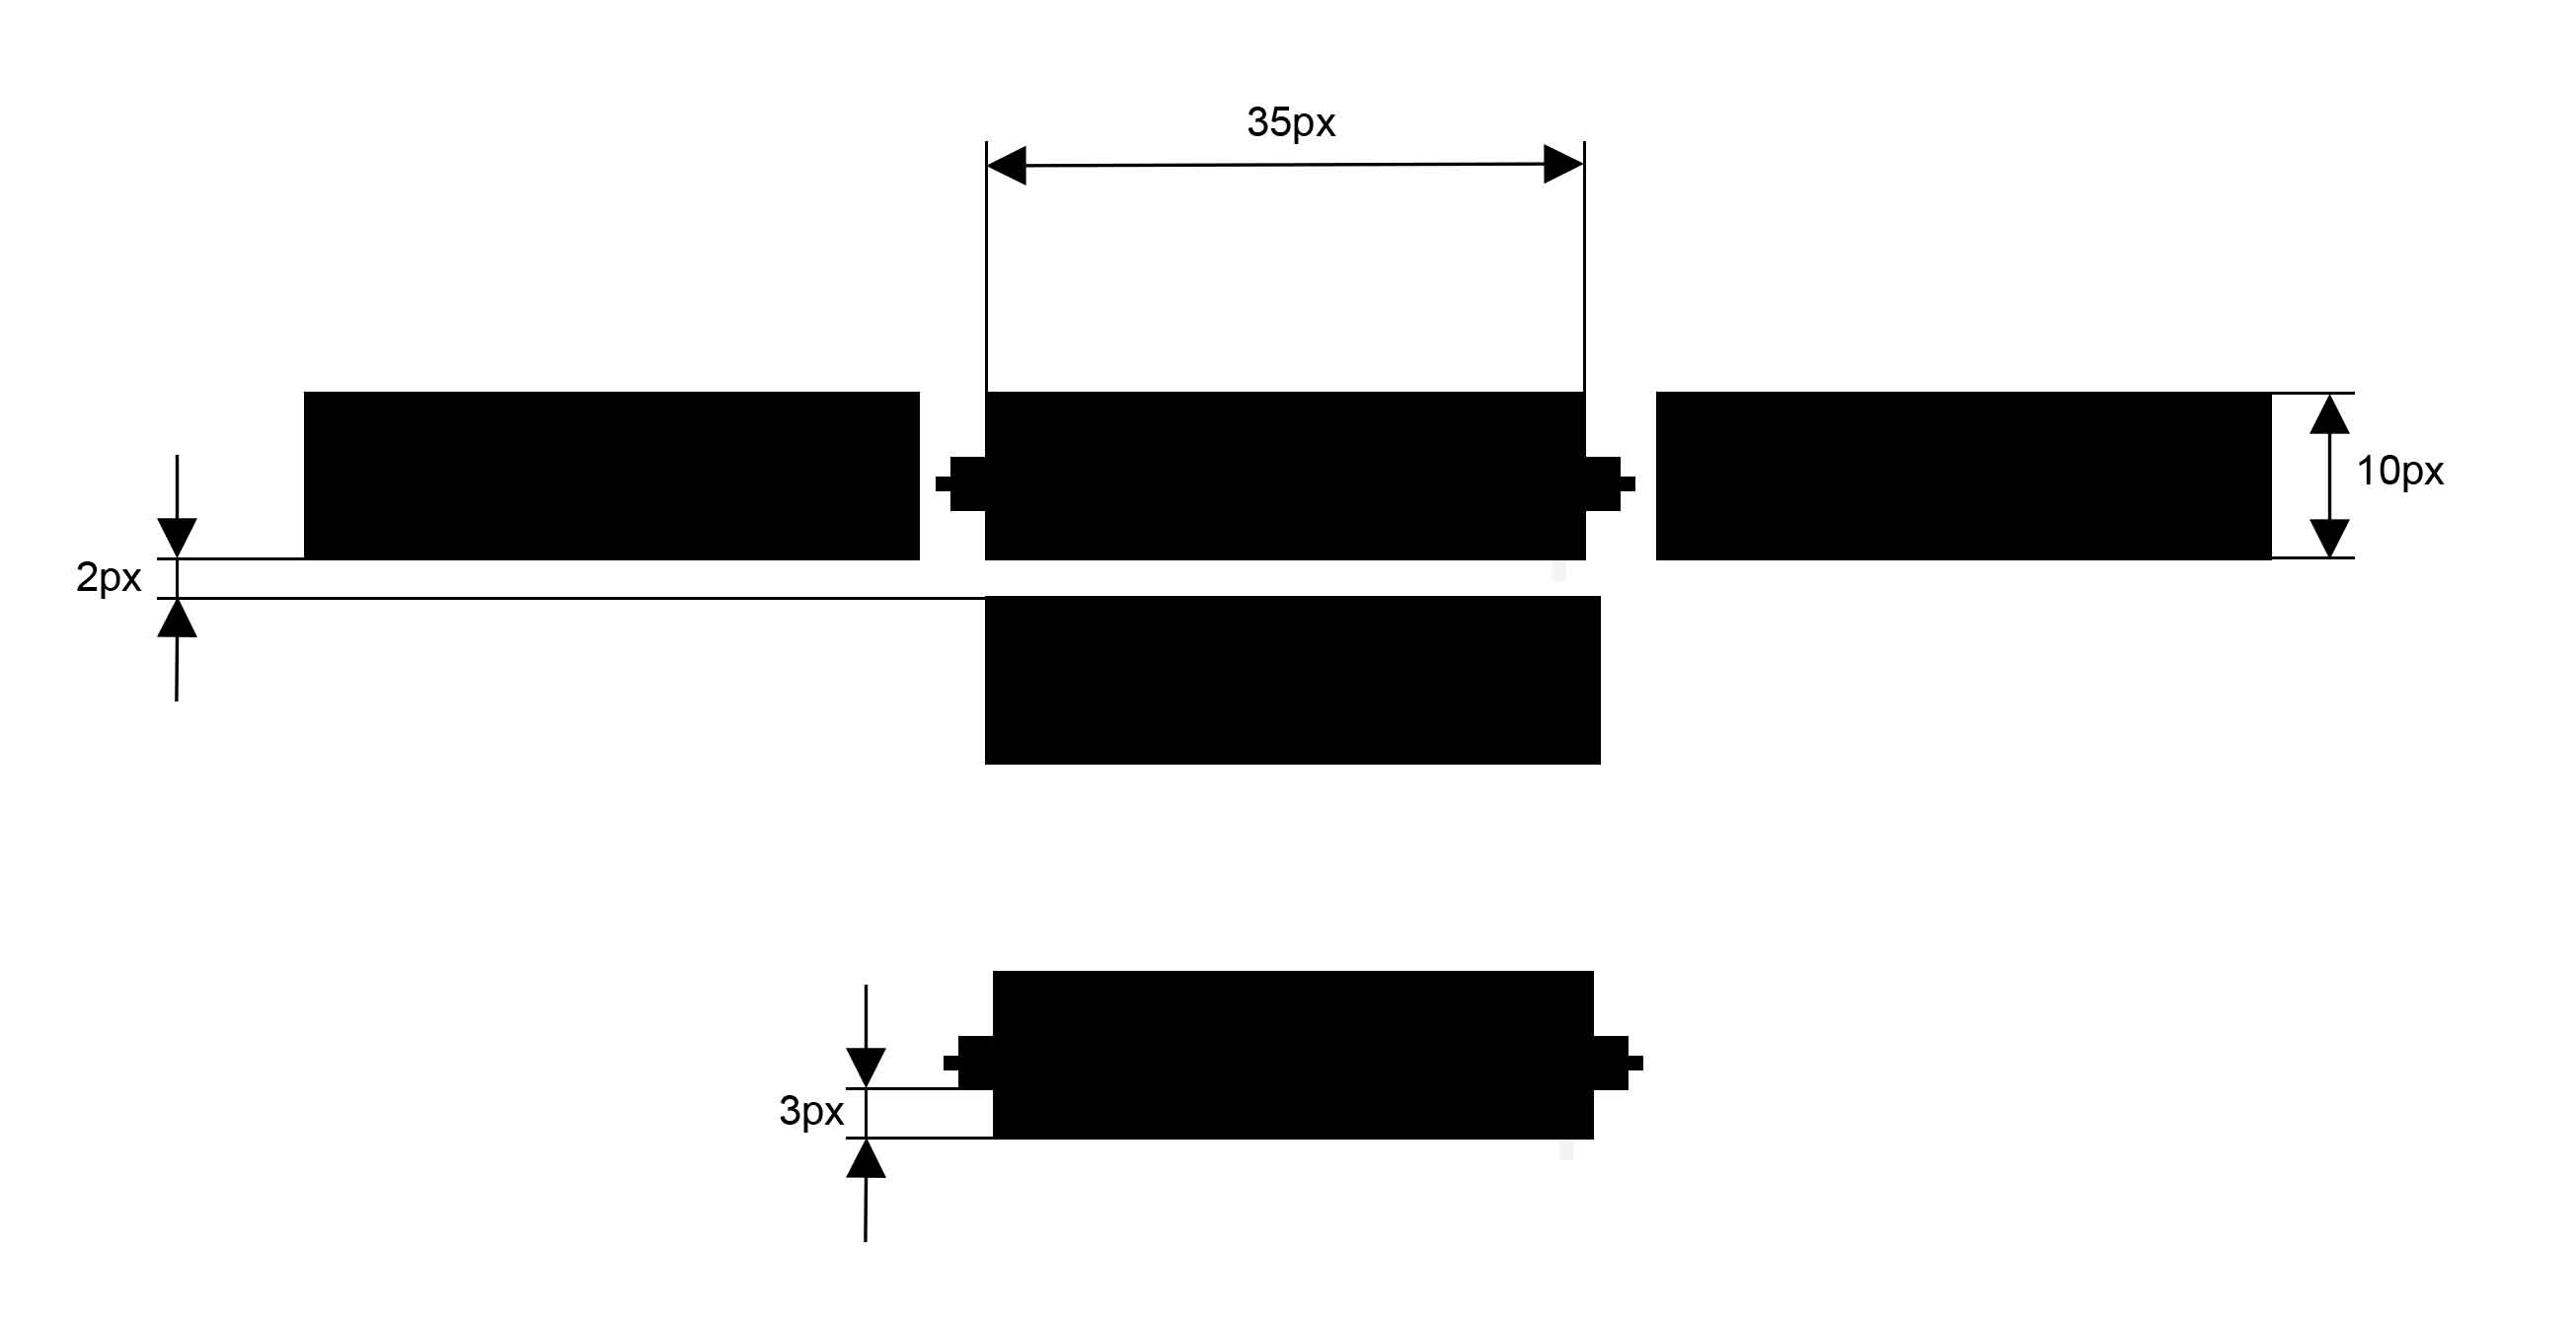
\includegraphics[width=1\linewidth]{measurement-and.jpg}
    \caption{First working AND gate}
    \label{fig:and-gate}
\end{figure}


A Petri dish, how likely is it to vary the resolution within the petry dish. how big is it 

how big is this pixel 

figure out the resolution. you can figure out the math quite easily. 

For this AND gate to be deployed in a Petri dish, how big does the Petri dish need to be. 

\begin{tcolorbox}[colback=red!5!white,colframe=red!75!black,title=NB!]
The size of the Petri dish is \textbf{assumed} to be unsubstantially larger than the size of the chemical circuit inside of it. Continuing from both sizes are referred to interchangeably.
\end{tcolorbox}


Ok, so here is the plan:
1. for the AND gate, figure out the constraints:
- min size of everything
- assumption is that there is no max size for the length as the waves just travel along. There is probably also no max width as the waves just expand, but there is probably a min width

2. Figure out the conditions for the AND gate to work in its smallest form, what are the conditions under which the AND gate would still work in the real world. For example, how close do they need to be in the real world before the light is not strong enough to keep them apart, maybe that's two-three pixels in the case of the simulation because 3 pixels are impossible to get across and two pixels are possible if the wave is focused towards the gap. 

In my case there is either max light or no light, so I need to be careful when I see how much light they are projecting in different spots.

intensity, angle, size of the light beam can influence the BZ reaction


some \todo{is it the same reaction} can be influenced by temperature \citep{yamada2022artificial}. The model they are using is a modified version of the Oregonator, that would be too much work for us. 

alright, first I need to find what the light-sensitive reaction is
then I need to inspect how they are shining the light, is it from above, from the side, is there multiple light sources.
then I need to inspect a data sheet for the diode they are using to see how the light shined everywhere differs, assuming the direct light below it is the maximum shined light, and I need to find a mathematical model that describes how the light around the diode becomes less.
what is the focus of that light?


Shining light on the BZ surface: \citep{barry1979methods}
The catalyst in these reactions is light, using light we can modulate the speed using $\Phi$.
A light bulb is shined over the Petri dish (fig. \ref{fig:light-over-petri})
\begin{figure}
    \centering
    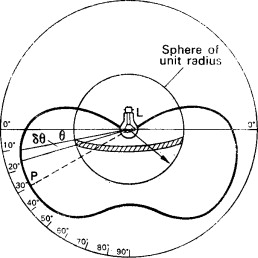
\includegraphics[width=0.5\linewidth]{sphere2.jpg}
    \caption{Light shined over a petri dish \citep{edwards_1970}}
    \label{fig:light-over-petri}
\end{figure}

Given multiple light sources, the total illumination $I_{\text{total}}$ at a point on a surface is the sum of the illuminations from each individual light source (fig. \ref{fig:light-flux-petri-dish}). The illumination $I_i$ from a single source at a given point is given by the inverse square law, adjusted for the angle of incidence $\theta_i$:

\[
I_{\text{total}} = \sum_{i=1}^{n} \frac{P_i}{4\pi r_i^2} \cdot \cos(\theta_i)
\]

where $P_i$ is the power of the $i$-th light source, $r_i$ is the distance from the $i$-th light source to the point, and $\theta_i$ is the angle between the direction of the $i$-th light ray and the normal to the surface. The cosine term $\cos(\theta_i)$ accounts for the angle of incidence, with the intensity contribution from the light source decreasing as the angle increases.



\citep{edwards_1970}

\begin{figure}
    \centering
    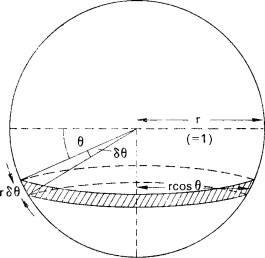
\includegraphics[width=0.5\linewidth]{sphere.jpg}
    \caption{Light flux at different parts of a Petri dish \citep{edwards_1970}}
    \label{fig:light-flux-petri-dish}
\end{figure}

This means that now we can use that in the simulation to simulate the imperfections of light sources. 

\todo{figure out how many light sources are used to illuminate a BZ reaction in a petri dish}

Now I have to figure out how exactly they shine the light to form an ihibitor path. Is it multiple bulbs? Is it just one bright bulb that is far away, so the $\theta$ is insignificant?

In real experiments, the chemical reaction that occurs on the gel surface is sensitive to light due to the specific catalyst used (Ru(bpy)$_3$SO$_4$). 
However, to observe and record the process, they need to use light to illuminate the gel, so that the camera can capture images. The experiment design, including time-varying intervals of different light intensities, allows them to balance between controlling the reaction and capturing the activity on the gel. \cite{TOTH20091605}

From what I see, they all project a single light bulb and then use a mask to have the shape they want projected, such that light does not kill off the reaction and there is light everywhere else. This is important to show how imperfections can affect the simulation. \cite{gorecki2003chemical}

This book \citep{cui2004synchronization}, referenced by \cite{gorecki2003chemical}, contains a similar setup and goes into more detail how they project the pattern onto the gel. 

Also the observation angle seems to change where we see the wave, idk if that is relevant. \citep{cui2004synchronization}.

Unfortunately, they do not specify how far away the camera is, but we can assume the came is far away, such that the angle of light projection is very close to $90^\circ$, so that would make the effect of the angle insignificant. However, we can still simulate that in our simulation to see what effect it would have if it were close to the medium; for larger circuits, this effect would be visible. Given a normal setup, what would be the maximum size of the Petri dish in a simulation before the effects of the light angle start to impact the simulation.

The next step is to assume a size; in the papers above they have the size of the AND gate coincidence deterctors used, so that can help me assume a relatively accurate size for the mapping from pixels in my simulation to a Petri dish. 

It is really challenging to find information on the exact distance the light source is from the Petri dish, but we are going to assume that the distance is 1m because that is how much it looks like from the diagrams they show where there are other objects like projectors and mirrors that are estimable. \citep{gorecki2003chemical}

Now I need to prove that for a small Petri dish, this would have an insignificant effect even in my simulation, but when we scale it, the effect would be very noticeable.

Now, this is just a simulation we are doing, so to get the mapping for a real Petri dish, we can use the dimentions of the gate in a Petri dish. 
In \cite{gorecki2003chemical} they specify the exact dimentions in mm of the collision detector inside of the Petri dish, which can be used to map it to the one in our simulation.
The distance between the active channel and the signal bar is 0.4 mm, which corresponds to exactly 2px in the simulation. 

from paper:
Both stripes are 2 mm wide, the signal channel is 10 mm long, and the detector part is 6 mm long. The gap between the signal and the detector channels is 0.4 mm. The light intensity was selected so that the non-illuminated parts of the membrane were excitable, whereas the excitations died in the illuminated areas. In the experiment, the light intensity was set at I ) 24 kLx as determined by a light metre (ASONE LM-332), and the temperature was 295 $\pm$ 1 K.


From the provided information in the paper and the datasheet for the JCD100V-300W halogen bulb, we have the following data:

\begin{itemize}
    \item Luminous flux ($\Phi$) as specified in the datasheet = 6600\, $\text{lm}$ \citep{fujilamp2024jdc}
    \item Light intensity (I) at the Petri dish = 24,000\, $\text{lux}$
\end{itemize}

Originally, we calculated the luminous flux using the estimated luminous efficacy of 17 $\frac{\text{lm}}{\text{W}}$ and the power of the bulb (P) as 300 W, which gave us:
\[
\Phi_{\text{estimated}} = \text{Power of bulb} \times \text{Luminous efficacy} = 300\, \text{W} \times 17\, \frac{\text{lm}}{\text{W}} = 5100\, \text{lm}
\]
However, this was an approximation. The datasheet for the bulb specifies a luminous flux of 6600 lm, which suggests that our assumption for the luminous efficacy was incorrect.

Using the inverse square law, which relates the light intensity (I) to the distance (r) from the light source, we have:
\[
I = \frac{\Phi}{4\pi r^2}
\]
Solving for the distance (r) with the correct luminous flux, we get:
\[
r = \sqrt{\frac{\Phi}{4\pi I}}
\]
Substituting the values from the datasheet and the light intensity measurement, we find:
\[
r = \sqrt{\frac{6600\, \text{lm}}{4\pi \times 24,000\, \text{lux}}}
\]
\[
r \approx 0.148\, \text{metres}
\]

Thus, the corrected distance from the light source to the Petri dish, using the accurate luminous flux from the datasheet, is approximately 0.148 metres or 14.8 centimetres. This distance is crucial, as it suggests that the light intensity measurement of 24 kLux is likely taken close to the Petri dish where the biological samples are studied, rather than at an arbitrary point close to the light source.

\begin{figure}
    \centering
    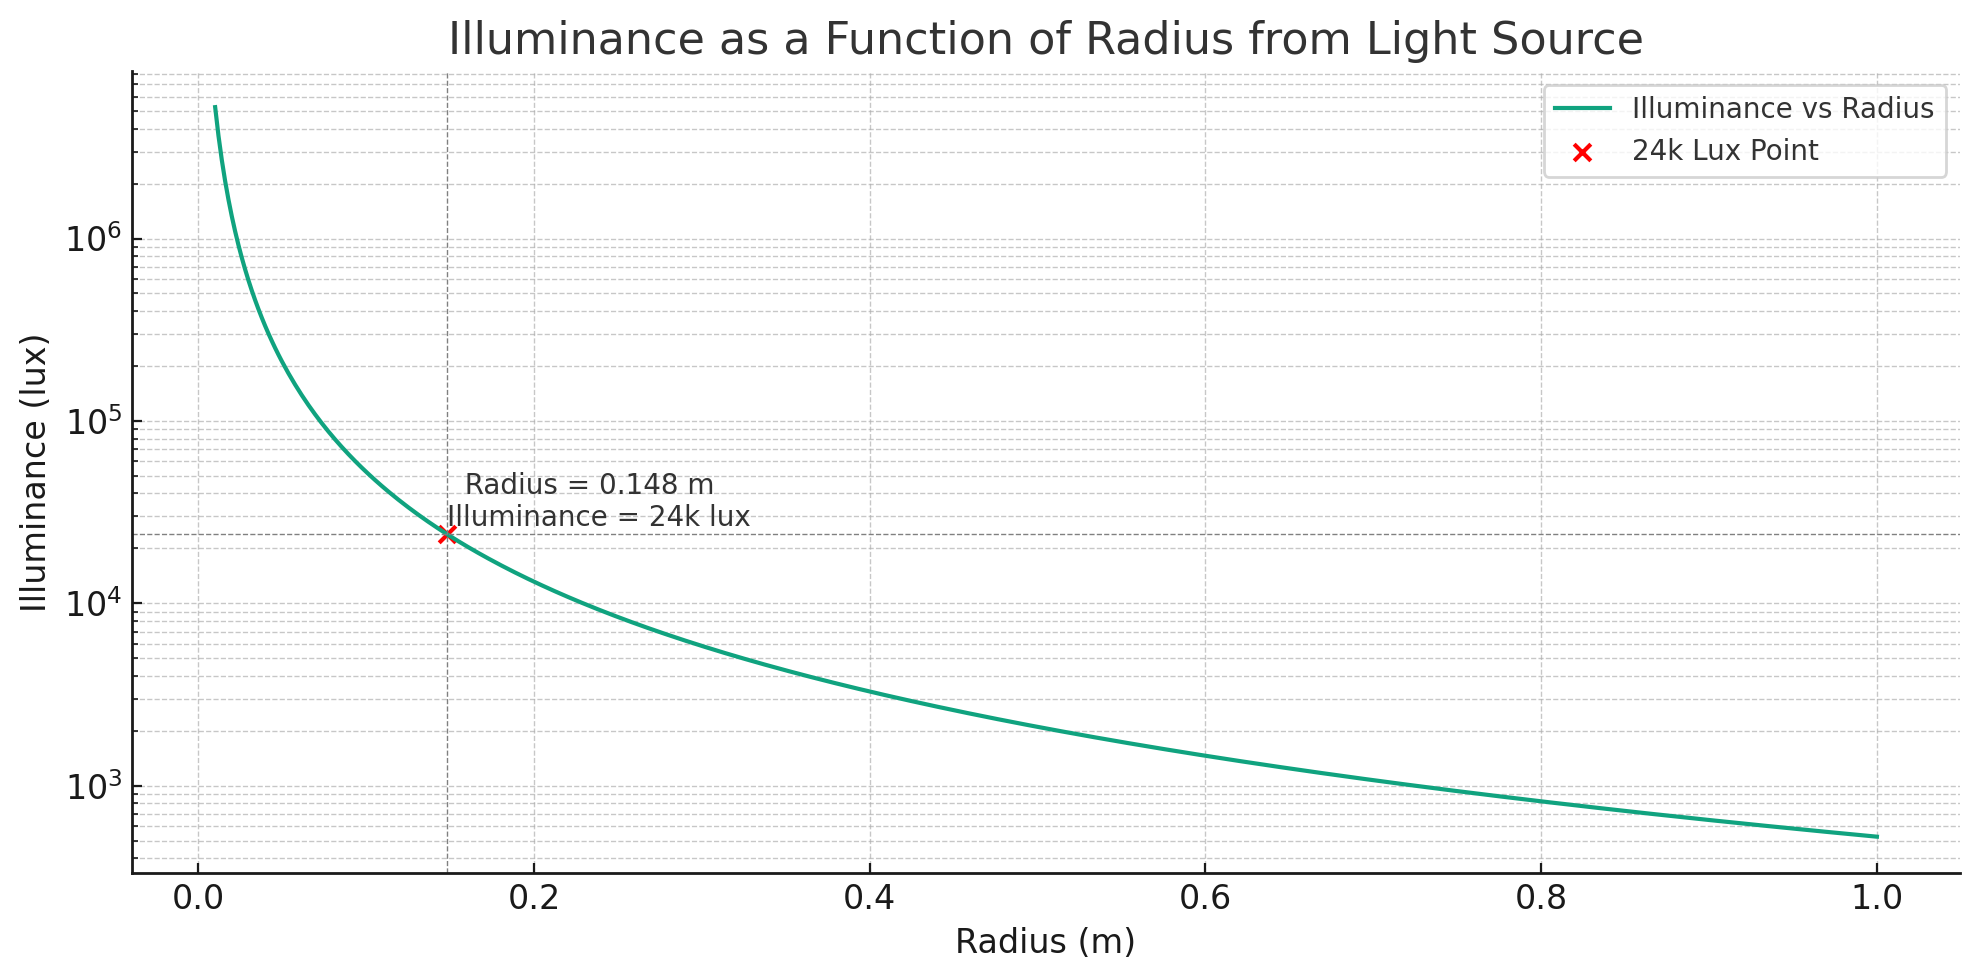
\includegraphics[width=\linewidth]{radius-illumination.jpg}
    \caption{Radius Illumination Graph}
    \label{fig:radius-illumination}
\end{figure}

In figure \ref{fig:radius-illumination} it is shown how the radius impacts the intensity at the light. This is necessary because it is not specified how they 

Given the luminous flux \( \Phi \) of the JCD100V-300W bulb as 6600 lumens, we can calculate the illuminance \( I \) at various distances from the light source. The illuminance is given by the formula:
\[ I = \frac{\Phi}{4\pi d^2} \]
where \( d \) is the distance from the light source in meters.

For distances of 10 cm, 12 cm, 18 cm, and 20 cm, the illuminance values calculated are:

\begin{itemize}
    \item At 10 cm: \( I \approx 52521 \) lux
    \item At 12 cm: \( I \approx 36473 \) lux
    \item At 18 cm: \( I \approx 16210 \) lux
    \item At 20 cm: \( I \approx 13130 \) lux
\end{itemize}

These values illustrate a significant change in illumination as the radius increases, indicating that the radius is a crucial factor in determining the intensity of light received at a point.

Concluding from these calculations, it is likely that the measurement of 24 kLux was made relatively close to the Petri dish. This is because the light intensity of 24 kLux is a practical measure for the conditions under which biological samples are typically studied. Measuring illuminance right next to the light source would yield an impractically high value, which is not as useful for experimental purposes. Hence, the measurement taken is more likely to be representative of the actual working conditions near the Petri dish.



Now I know how far away the Petri dish is from the light source, but I still do not know the size of the Petri dish they used. 
\section{Coincidence Detector Size Limitations}
In the setup \citep{gorecki2003chemical} they specify a signal channel of 10cm and a membrane filter of 2.5cm. The filter applied is usually smaller than the Petri dish itself, but for now we can just look at the dimentions  we specified at \todo{reference the place where you said all the cm used in the dish}. 


Given the following mapping from real life measurements to simulation pixels:
\begin{itemize}
    \item Stripe width: \(2 \text{ mm} = 10 \text{ px}\)
    \item Channel gap: \(0.4 \text{ mm} = 2 \text{ px}\)
\end{itemize}

We can establish a scaling factor for the conversion from millimeters to pixels.
For the stripe width:
\[ \text{Scaling factor} = \frac{10 \text{ px}}{2 \text{ mm}} = 5 \text{ px/mm} \]

For the channel gap:
\[ \text{Scaling factor} = \frac{2 \text{ px}}{0.4 \text{ mm}} = \frac{2 \text{ px}}{\frac{2}{5} \text{ mm}} = 5 \text{ px/mm} \]

Thus, both measurements confirm the same scaling factor. Using this consistent scaling factor, we can convert any measurement from millimeters to pixels.

Using this scaling factor, we can convert any measurement from millimeters to pixels.
For a dimension of \(10 \text{ mm} \times 4.4 \text{ mm}\), the conversion would be:

\begin{align*}
\text{Width in pixels} &= 10 \text{ mm} \times 5 \text{ px/mm} = 50 \text{ px} \\
\text{Height in pixels} &= 4.4 \text{ mm} \times 5 \text{ px/mm} = 22 \text{ px}
\end{align*}

Thus, a real-life size of \(10 \text{ mm} \times 4.4 \text{ mm}\) would map to a size of \(50 \text{ px} \times 22 \text{ px}\) in the simulation.


Realistically, we only care about the size of the circuit inside of the Petri dish, so we don't really need to know the actual size of the Petri dish for this imperfection. 

Next thing is to put the imperfection in the simulation with jsut an and gate. To do that, I need to come up with a formula about plugging in a pixel and getting out the illumincation percentage. 
The percentage is basically the $\cos\theta$ as it is 0 when the angle is $90^\circ$.
let's assume a parallel light source is max intensity and an angle of 0 is no intensity at all, so in the formula we would plug in $\phi=0.054$ for when it's active and $\phi=0.0975$ when it's passive. Active means no light, passive means a lot of light, so when the light source becomes weak at a point, that would mean thath $\phi$ becomes more active. 
let's come up with a formula in mm that tells us when we move 1mm from the center of the petri dish where the light is most intense, what angle is that. That should be pretty simple, we have a right triangle, 
\begin{figure}
    \centering
    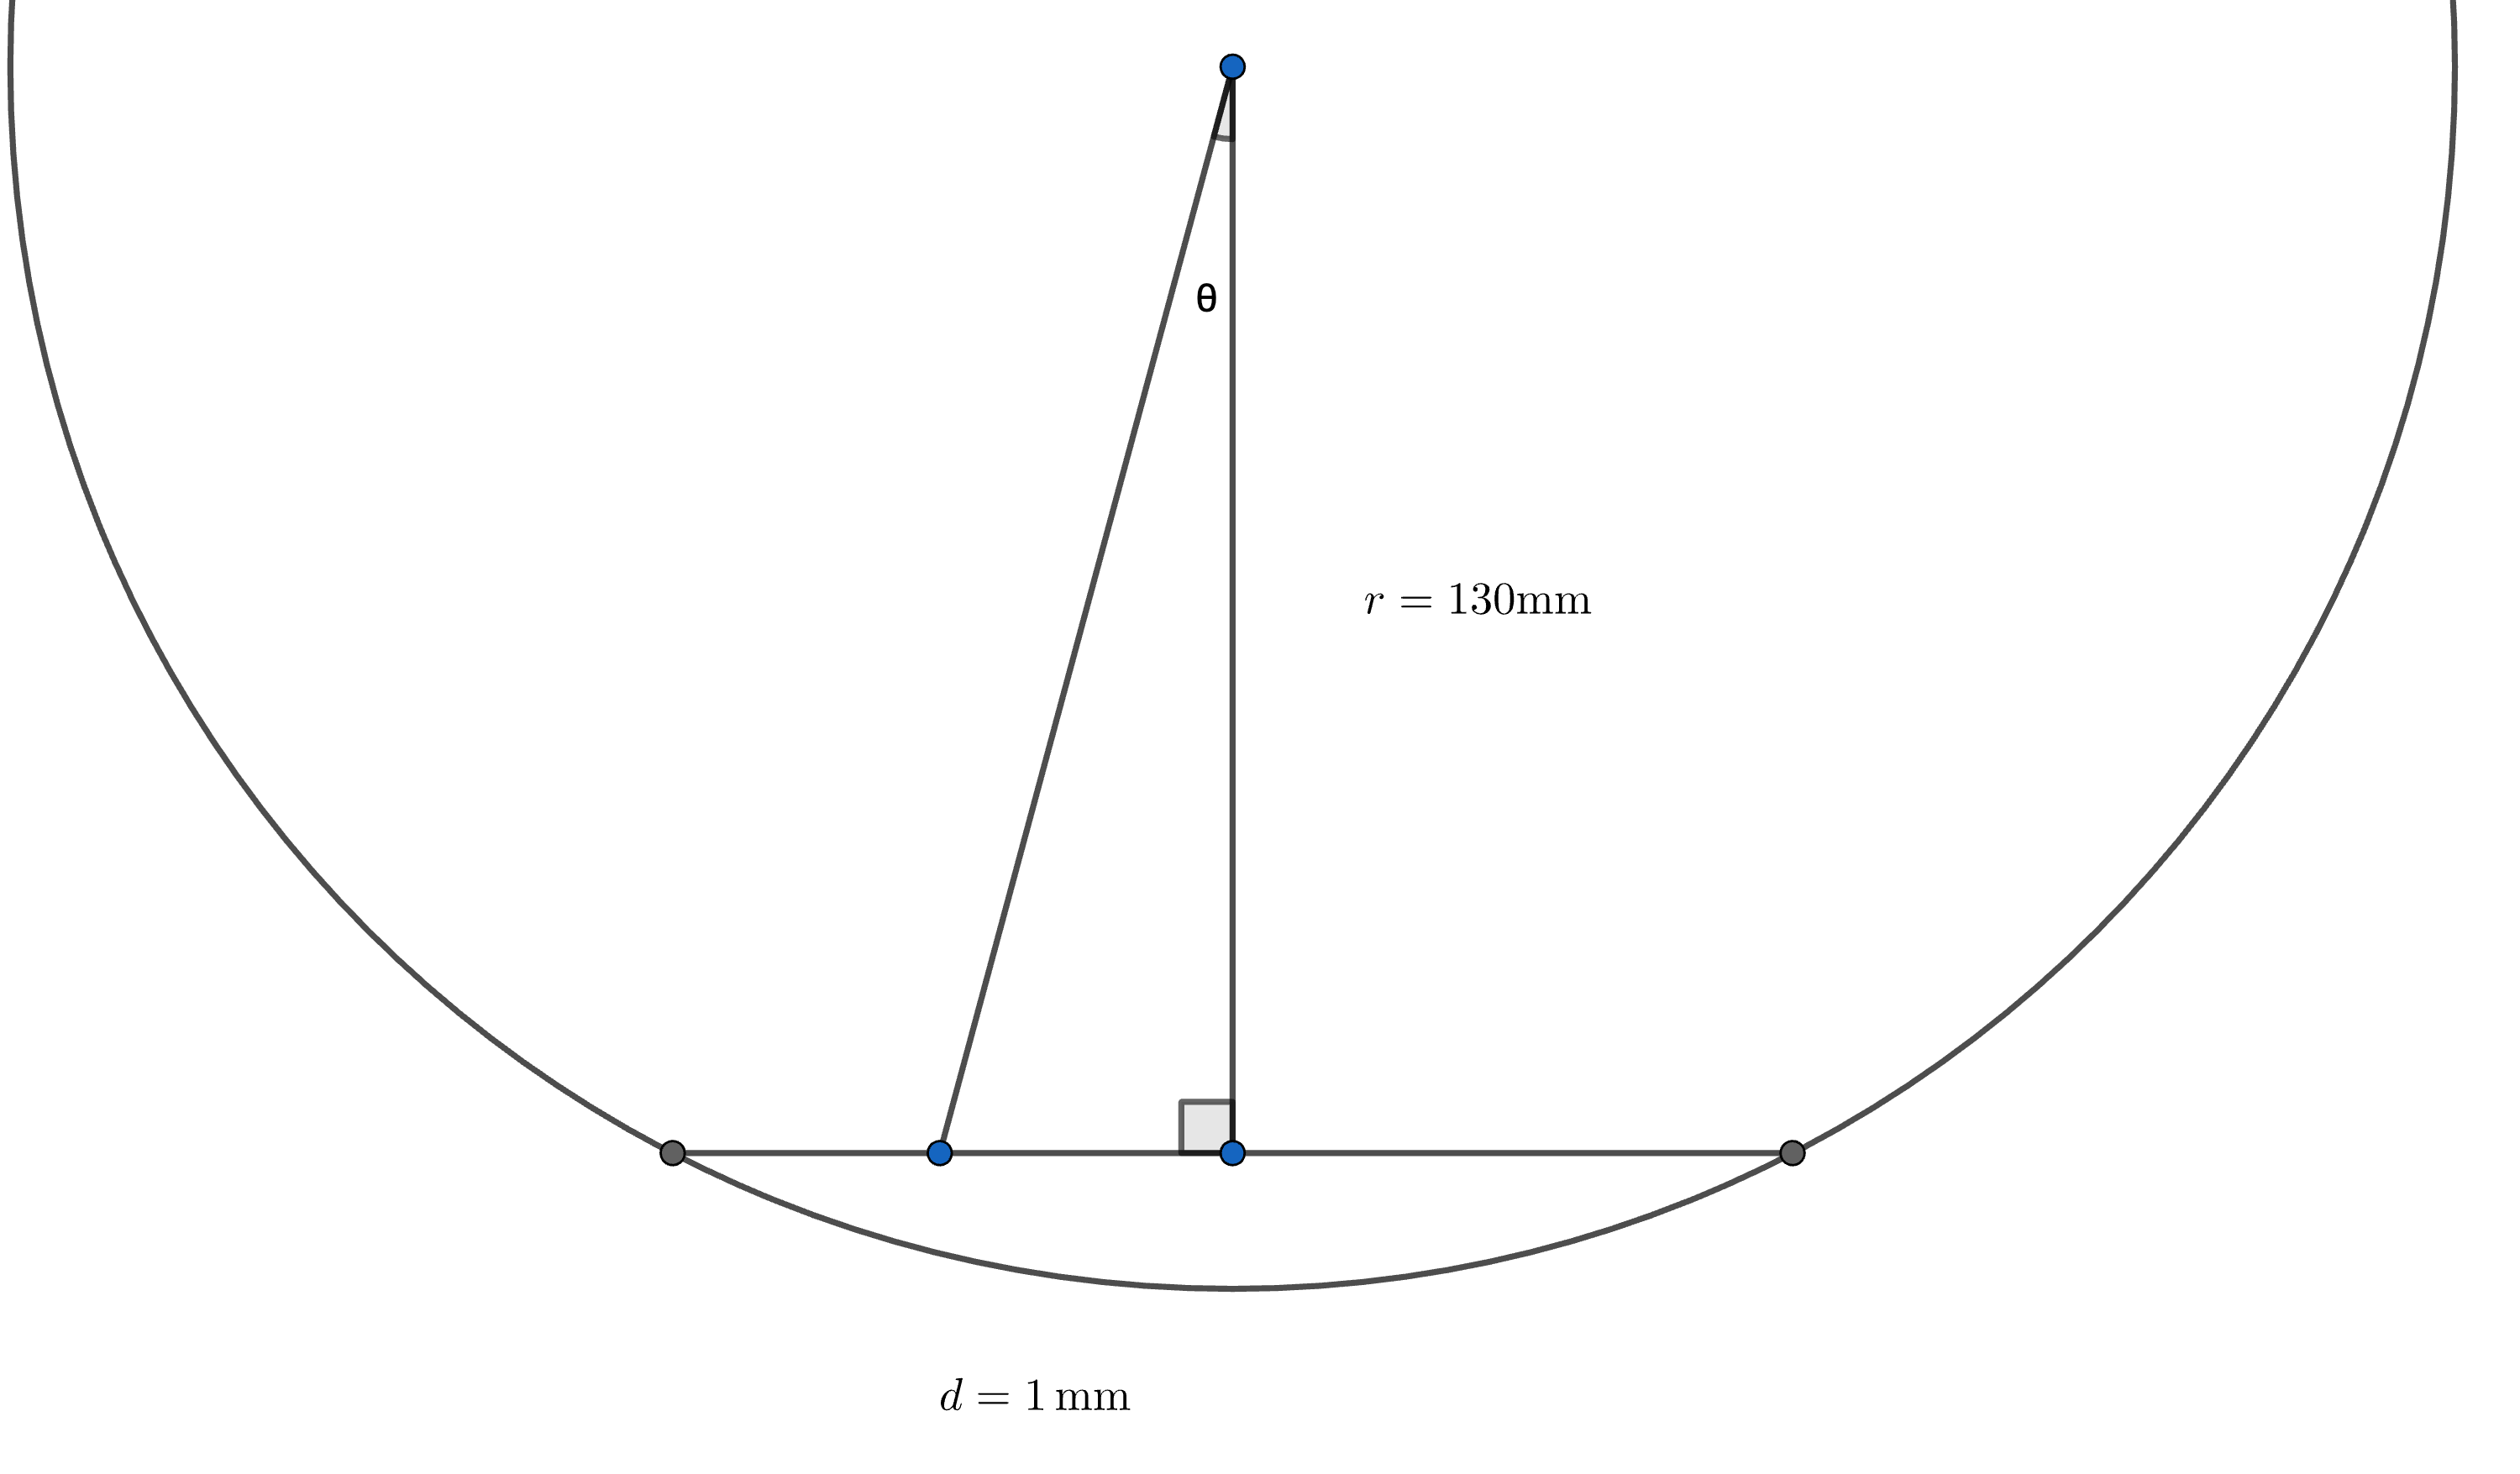
\includegraphics[width=1\linewidth]{geogebra-export (1).png}
    \caption{Illustration of finding the angle $\theta$}
    \label{fig:finding-theta}
\end{figure}

i made a bad assumption, i thought when we get the 0.44 angle for a 1mm distance, we can just get 0.88 for 2mm, which is prolly not true, we have to find the angle every time

To calculate the angle \( \theta \) for any given radial distance \( r_c \) from the center of the Petri dish, we convert the pixel distance \( p \) to millimeters using the scaling factor \( s \) (in px/mm):

\[ r_c = p \times s \]

The angle \( \theta \) is then found using the arctangent function with respect to the height \( h \) of the light source above the center of the Petri dish:

\[ \theta = \arctan\left(\frac{r_c}{h}\right) \]

The percentage of illumination \( I_p \) at this radial distance is given by the cosine of \( \theta \):

\[ I_p = \cos(\theta) \]

Since \( \cos(\arctan(x)) \) simplifies, we can express \( I_p \) directly as:

\[ I_p = \frac{1}{\sqrt{1 + \left(\frac{r_c}{h}\right)^2}} \]

This formula calculates the percentage of illumination at a point \( r_c \) millimeters from the center, assuming the light intensity directly beneath the source is 100%.


From manual tests with illumination, the circuits start behaving not as expected even with illumination percentages less than 0.99 because the simulation is very sensitive to changes in light intensity as it relies on a manifold of light-affected microinteraction. Using this value of 0.99, we can see at what size of the Petri dish do we start to see values below 0.99. We can calculate that and then confirm in the simulation. 


I debugged the nonworking thing with a debug variable inside the metal function controlled by my mouse. 
I just verified that the simulation does break once the illumination reaches 0.99. I did not get much value from putting this inside the simulation, more like, oh yeah, I am correct.
I could have verified that 0.99 is the threshold by just running 
it.

I verify using a simulation that if the circuit is too big, a single light source might not be enough to illuminate the whole area relatively evenly and even light perturbations in the light are going to disrupt larger circuits. 
What can be done is to make the circuit different the further away it is from the source, which would involve different dynamics that work under different lighting conditions. This is infeasible to do practically as it so highly depends on the light source. 

The 0.99 is kind of sus, I still need to figure out a lot of things like a more optimal mapping from the real-life illumination intensity and the mathematical formula in the Oregonator model. I think my mapping is okay because $\phi_{\text{active}}$ is what it is and $\phi_{\text{passive}}$ can be moved even further, I just interpolate between these values, maybe there is a better way to simulate it. The problem with my simulation is that it does not matter how strong the light source is, you can put the whole sun over the Petri dish, the illumination at the angle is still going to be 0.99 of the original, I need a better way to simulate it that can also input the parameters of the light source, so it's not just about the strength. I need something like a threshold for when the light intensity is so strong that nothing can pass through. That is also a problem, however, because the actual circuit relies on the gaps being not too illuminated, so that the activator chemical can diffuse towards another part of the surface. It's again difficult to come up with a model. 
So that means a more powerful light bulb might create different things for different illuminations, but it might not work if the Petri dish is directly under it as it might create too much illumination and prevent the waves from crossing boundaries. \textit{I don't know}. So the 0.99 is only true when the assumption that $\phi_{\text{active}}$ is equivalent to the Hallogen light bulb of 300W used directly above it.

Maybe, just maybe, the relationship is not linear as I assume, but logarithmic, so as the illlumination in real life decreases, that creates a logarithmic decrease in $\phi$ from $\phi_{\text{active}}$ to $\phi_{\text{passive}}$, so it might not be as sensitive to the small changes in light as I assume. \todo{To resolve this, how did the var values come about }

In the simulation very small changes in light intensity were found to very significantly affect the propagation delay of the activator signal. This is crucial for the operation of the circuit. These circuits do not have any way of synchronisation other than propagation delay, which means even the slightest change in light intensity is going to affect the speed of propagation and the whole circuit would break. This is more important for bigger circuits like the ones built by \cite{StovoldJames2019RaGI}, that rely heavily on exact propagation. 
In my simulation it was very sensitive to the illumination changes, maybe in real life as long as it's more illuminated than some \textit{threshold}, then it doesn't matter for the simulation. I need to do more digging to figure out what to do from here.

\section{Temperature}
Let's examine how temperature affects reaction diffusion. 


say im assuming the light bulb is not using soft light, it has not piece of paper so inverse square law is fine. 


we're looking at a paper working with old technologies. 
let's use an LED panel, uniform light, scale better.

Bell curve for light distribution of light. 

how does the phi relate to the real world.

dig into the oregonator model, what do they define as phi?exitability? what is the mapping? it's nonlinear.

temperature is not a great route, what effect would dust have on the wave propagation. 

exploring how does different light source magnitudes get affected by a sheet of paper ? less useful....




focus on the large petri dish. 


why are you measuring the pixels? 

dont talk about papers, talk about research 


general introduction - what is this, background \& literature review, what have other people done , why is this important.  
james has done this, how possible is this in real life. 
aims and objectives are next - i wanna look.
 specify them





then we look at the results, what is the meat of what ive found.


then there is a discussion section , opposite of backtournd and lit review, now we go back out. 
place our findings in the context of our literature, how does thi simpact, tha'ts where my views come in, 
scientifically... how realistic is it? 
now that we know this new piece of information 


conclusion \& evaluation

what you've done, what you've larned . reflection manner shows you what you've learned.

give it some reasonable name - related to what im doing. 




Ok, I need to understand how illumination maps to $\phi$. For that I need to understand the Oregonator model


that's it, we need to find the minimum and maximum reaction rates in real life reactions. 
we already have a minimum and maximum in the simulation ,we can check if they behave the same way. if they do, that's our threasholds, then we need to find an appropriate function that describes a similar relationship and we found it


The main idea is that when there is no activator in the solution,  \citep{reddy1995effect}



\subsection*{Beer-Lambert Law for Absorption}
\todo{Move to future work, looking at phi act and phi pass are related, atm we are varying passive, but activve would change as well, atm we are making the assumption no light is going through ,but could calculate their relationship using some fomrula for absorbtion like this }
The Beer-Lambert Law describes how the intensity of light decreases as it passes through an absorbing medium:
\[ I = I_0 \cdot e^{-\alpha \cdot l} \]
where:
\begin{itemize}
    \item \(I_0\) is the initial light intensity before hitting the OHP sheet.
    \item \(I\) is the light intensity after passing through the material.
    \item \(\alpha\) is the absorption coefficient of the OHP sheet material.
    \item \(l\) is the thickness of the OHP sheet.
\end{itemize}

For our calculations, we assume an absorption coefficient \(\alpha = 1\ \text{m}^{-1}\) and a thickness \(l = 0.004\) meters (4 mm).

\subsection*{Fresnel Equations for Transmission}
The Fresnel equations determine how much light is transmitted and reflected at an interface, depending on the angle of incidence. For non-polarized light and considering both s-polarized and p-polarized components, the average transmission \(T\) can be approximated by:
\[ T = \frac{T_s + T_p}{2} \]
where \(T_s\) and \(T_p\) are the transmission coefficients for s-polarized and p-polarized light, respectively. These coefficients are calculated using the refractive indices of the air (\(n_1\)) and the OHP sheet material (\(n_2\)), and the angle of incidence \(\theta_i\).

\subsection*{Calculation at 45 Degrees Angle of Incidence}
At a 45-degree angle of incidence, we calculated the transmission coefficients for s-polarized and p-polarized light, and found the average transmission \(T\) to be approximately 0.950. This indicates that about 95\% of the light is transmitted through the OHP sheet at this angle.

Combining the effects of absorption and transmission, the final intensity \(I_{\text{final}}\) of light after passing through the OHP sheet and considering the angle of incidence is given by:
\[ I_{\text{final}} = I_0 \cdot e^{-\alpha \cdot l} \cdot T \]

Substituting the given values and assumptions, we find:
\[ I_{\text{final}} \approx 0.946 \]
This result indicates that the combined effect of slight absorption by the OHP sheet and the reduction in transmission due to the 45-degree angle of incidence leads to a final light intensity of approximately 94.6\% of the initial intensity.

These calculations demonstrate the importance of considering both material properties and geometric factors, such as the angle of incidence, when modelling the transmission of light through materials in experimental setups.



\todo{the diffusion assumes 100\% goes through at the centre of the  light source, it's more like 99\% or something}

\chapter{Experiments}
Here $\phi_{passive}$ is measured at different values because that is the value controlling the illuminated area, which makes the circuit there ``passive'' \todo{figure out if that's how quotes should be or reveresed}. This simulates less illumination of light at the diode, altering its behaviour.
\section{Measuring $\phi_{min}$, $\phi_{max}$ and propagation time for the diode at different light conditions}


During the evaluation of $\phi_{min}$, $\phi_{max}$, the diode had to be tested from numerous directions to determine the minimum and maximum values of $\phi_{passive}$ where it still functions correctly as a diode, which means that it passes waves from right to left, but never from left to right. As we approach the limits, new cases start appearing where the wave becomes able to pass through from a very specific angle that changes as we change the phi value, making it impossible to automatically test, so manual testing was needed to verify if the diode works in every single use case for the limit phi values. Also, the minimum and maximum values start to highly depend on the testing conditions, and whether the diode works or not starts to depend on how you are using it; for example, do you start a wave right at the diode? If not, what is the minimum distance the diode has to work for? This greatly changes the minimum and maximum phi values. 

Results of measurement: 
\begin{itemize}
    \item $\phi_{max} = 0.106127$
    \item $\phi_{min} = 0.09555$
\end{itemize}

That is, as long as $\phi_{min} < \phi_{passive} < \phi_{max}$, then the diode will function as expected, even though the propagation time would still be affected (as seen in Figure \ref{fig:phi_passive_propagation_times}), causing synchronisation problems in larger circuits.


The way the experiment was set up was that a diode was set up in Figure \ref{fig:diode_experiment} where a wave was launched 25 px from the diode to allow it to pass through the diode and reach a small white flag where the wave is expected and the experiments are evaluated. A step in the diagram means one simulation pass. The parameters of the experiment were the following:
\begin{itemize}
    \item Number of $\phi_{passive}$ values: 30, of which only 19 succeeded, the remaining 11 could not pass through the diode due to the parameter being too out of range.
    \item Interval size: 0.0013448276
    \item Number of runs per $\phi_{passive}$ values: 7
    \item $\phi_{start}$: 0.08066608
    \item $\phi_{end}$: 0.121010914, never reached because once a wave passes through the diode, the concentration no longer reaches zero fully and that leaves a very small amount of inhibitor at the diode and due to the borderline value of $\phi_{passive}$ the next waves never manage to penetrate to get measured, so the highest measured value for $\phi_{passive}$ is 0.10487298
    \item Wave start: 39px before diode, arbitrary distance to allow the wave to form.
    \item Wave measure: 31px after diode, arbitrary distance.
    \item $dt$: 0.001, also serves as a reference point for the amount of steps.
    \item Measurement interval: about every 50 steps, depending on the GPU frame rendering schedule
\end{itemize}

It is possible to run the experiment much more accurately, eliminating the need for multiple runs for the same $\phi_{passive}$ value we measured at every step and did not simulate another step in the simulation until the measurement was complete. However, that would drastically slow down the experiment, making it run for hours instead of minutes. For the purposes of merely showing that the propagation changes along with the slope, it was enough accuracy, so the faster and more inaccurate solution was chosen.

\begin{figure}
    \centering
    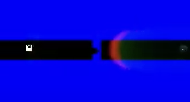
\includegraphics[width=0.5\linewidth]{diode.png}
    \caption{Diode Experiment}
    \label{fig:diode_experiment}
\end{figure}

So, I found the following limitation while working with the simulation. Due to the act that in metal sampling is a rendering operation, it cannot be done during the computation of the simulation. That means that I would have to synchronise it to run with rendering speed, but that would make the simulation too slow to run many experiments. It uses the step speed of the simulation, 1 frame = about 150 steps in the simulation. This is still accurate enough. I ran at $dt=0.001$.

\subsection{Results}

The results of the experiment can be seen in Figure \ref{fig:phi_passive_propagation_times}. The propagation time decreases as there is less light, indicated by the decrease in the value of $\phi_{passive}$ and the reverse. This is to be expected, as a lower value brings it closer to $\phi_{active}$ (darkness), and illumination is an inhibitor. 
The reason the circuit has a higher tolerance to less light, compared to more light, is because the diode is much more resistant in the reverse direction as the wave has to go through a reverse triangle \todo{figure out how the point thing is called}. 
The diode also has a high tolerance to $\phi_{passive}$ increasing due to an additional spike added to the diode, which helps weaves to cross the gap easier, even when there is more light. \todo{measure without the spike, how bad is it}. The reason for $\phi_{max} < \phi_{end}$, meaning the diode was still letting the wave through left to right and not right to left at $\phi_{end}$, but it was not at other angles when tested, so the experiment measured propagation time, but the diode was only partially functional at these values

\begin{figure}
    \centering
    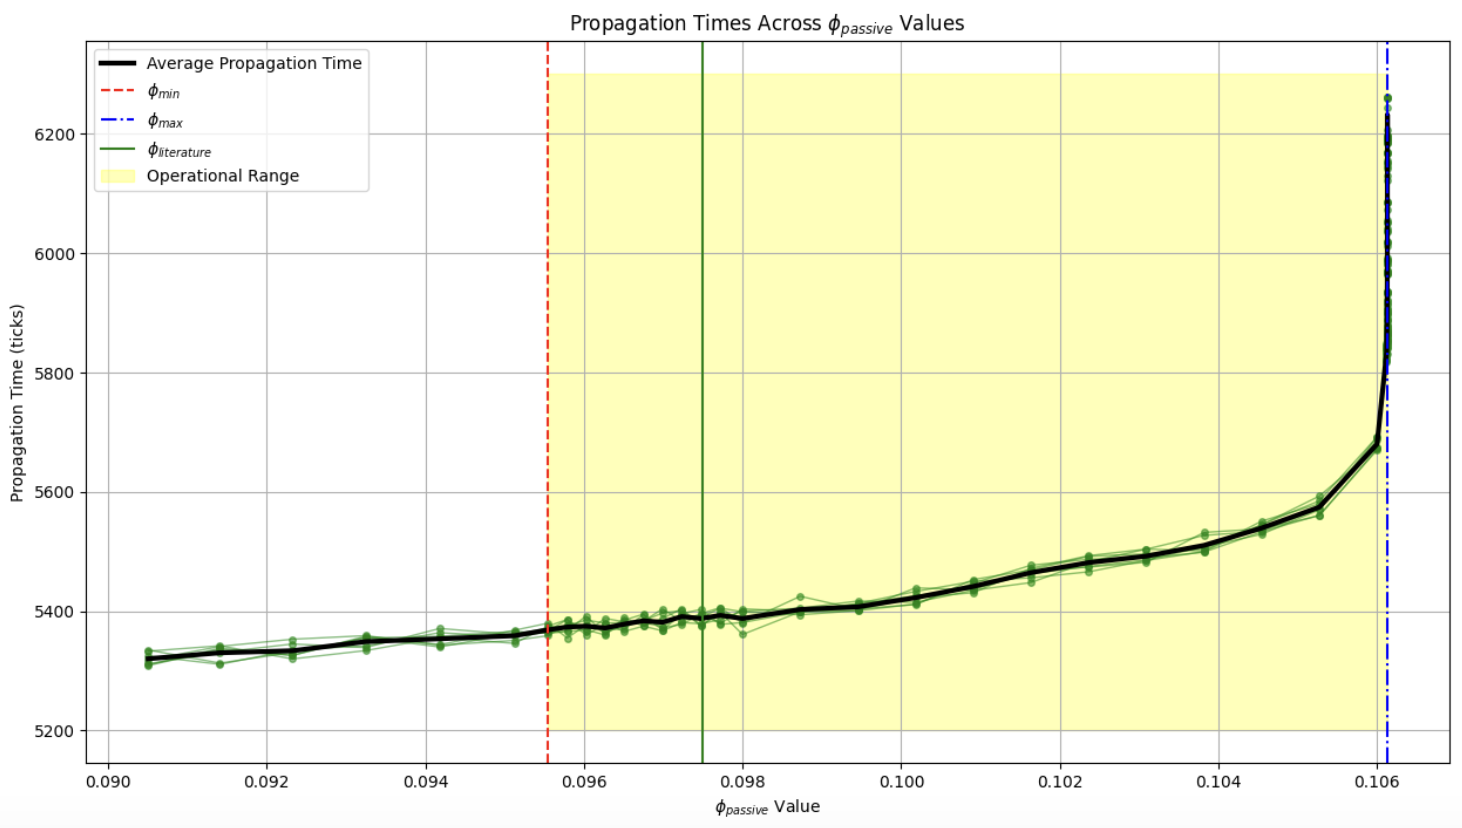
\includegraphics[width=\linewidth]{Screenshot 2024-03-09 at 10.35.01.png}
    \caption{Propagation times for various $\phi_{passive}$ values within the limits of $\phi_{min}$ and $\phi_{max}$, illustrating the experimental outcomes of testing a diode in a Belousov–Zhabotinsky reaction. Each point represents a propagation time measurement for a given $\phi_{passive}$, with the average propagation time across measurements shown by a thicker black line. The shaded area between $\phi_{min}$ (red dashed line) and $\phi_{max}$ (blue dashed line) highlights the range where the diode works correctly, with the optimal $\phi$ marked by a solid green line.}
    \label{fig:phi_passive_propagation_times}
    
\end{figure}

\begin{figure}
    \centering
    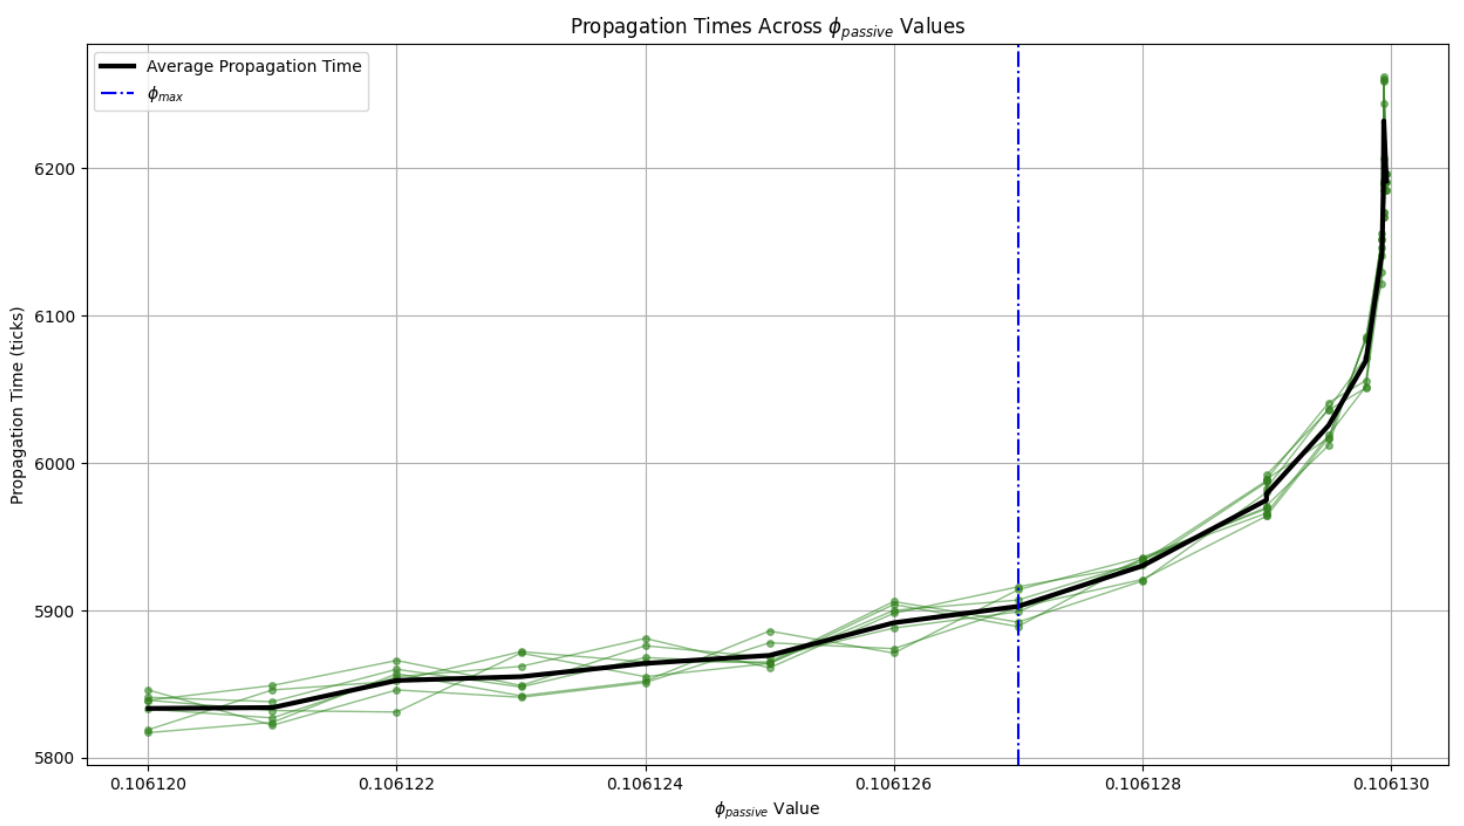
\includegraphics[width=1\linewidth]{Screenshot 2024-03-10 at 07.50.59.png}
    \caption{Propagation times at $\phi_{max} - $}
    \label{fig:phi_passive_propagation_times_detail_max}
\end{figure}



\begin{figure}
	\centering
	\begin{subfigure}{0.24\textwidth}
		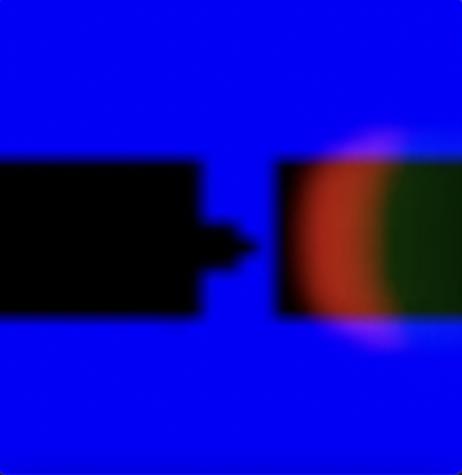
\includegraphics[width=\linewidth]{diode/easy/Screenshot 2024-03-09 at 16.21.56.png} 
	\end{subfigure}
	\begin{subfigure}{0.24\textwidth}
		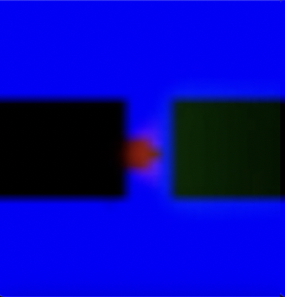
\includegraphics[width=\linewidth]{diode/easy/Screenshot 2024-03-09 at 16.22.24.png} 
	\end{subfigure}
    \begin{subfigure}{0.24\textwidth}
		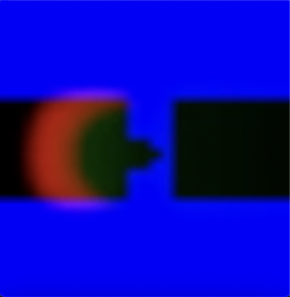
\includegraphics[width=\linewidth]{diode/easy/Screenshot 2024-03-09 at 16.22.35.png} 
	\end{subfigure}
    \begin{subfigure}{0.24\textwidth}
		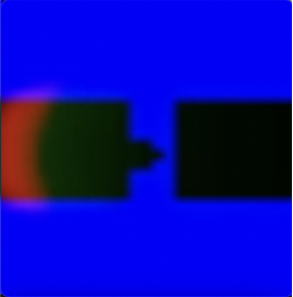
\includegraphics[width=\linewidth]{diode/easy/Screenshot 2024-03-09 at 16.22.45.png} 
	\end{subfigure}

	\begin{subfigure}{0.24\textwidth}
		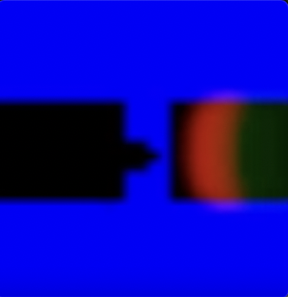
\includegraphics[width=\linewidth]{diode/hard/Screenshot 2024-03-09 at 16.23.41.png} 
	\end{subfigure}
	\begin{subfigure}{0.24\textwidth}
		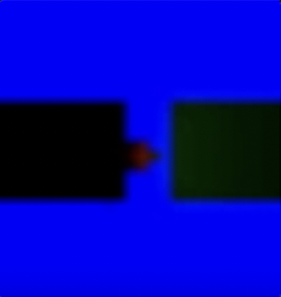
\includegraphics[width=\linewidth]{diode/hard/Screenshot 2024-03-09 at 16.23.48.png} 
	\end{subfigure}
    \begin{subfigure}{0.24\textwidth}
		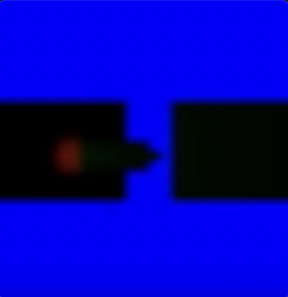
\includegraphics[width=\linewidth]{diode/hard/Screenshot 2024-03-09 at 16.23.55.png} 
	\end{subfigure}
    \begin{subfigure}{0.24\textwidth}
		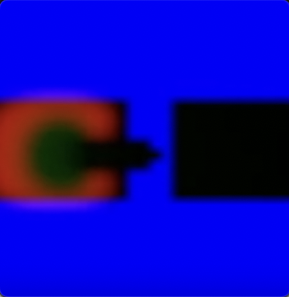
\includegraphics[width=\linewidth]{diode/hard/Screenshot 2024-03-09 at 16.24.01.png} 
	\end{subfigure}

	\caption{Comparison of two waves passing through a diode. Above $\phi_{passive} = \phi_{literature}$, below $\phi_{passive} = \phi_{max}$. Both have different propagation speeds, so they have been equalised for the purpose of comparing their interaction with the diode side by side. The second wave takes substantially more time to form and is about 700 time steps slower as seen in Figure \ref{fig:phi_passive_propagation_times_detail_max}, which is quite a lot in such simulations.}
	\label{fig:comparison_diode}
\end{figure}